\section{Unavoidable Hazards of Bureaucracy\label{sec:unavoidable_hazards}}

In a bureaucracy there are certain challenges that cannot be avoided. The value of recognizing them is to understand that what you're experiencing isn't an anomaly. The problem isn't unique to you, your circumstances, your coworkers, or the organization. The cause is the combination of all those factors.

\ \\

\textbf{Separation of responsibility and accountability}. \\
Each bureaucrat in an organization has responsibilities associated with their role. The ability to complete the tasks associated the role are not wholly within the scope of the bureaucrat's control. Even if there is a desire for action, the action might not be immediately feasible because of a dependence on another person or process. 

\ \\

\textbf{Appreciation for being an effective bureaucrat is rare.}\\
If you do your job well, at best no one will notice.

``No one [thanks teachers] for policing cheating. Not the cheaters, not the honest students who feel inconvenienced and mistrusted, and certainly not the school [administrators] who have to process academic dishonesty paperwork.''\footnote{https://dynomight.net/teaching/}

The number of thank you cards sent to \href{https://www.fda.gov/}{Food and Drug Administration} meat inspectors, \href{https://www.osha.gov/}{Occupational Safety and Health Administration} regulators, \href{https://www.fcc.gov/}{Federal Communications Commission}, \href{https://www.ftc.gov/}{Federal Trade Commission}, and \href{https://www.sec.gov/}{Securities and Exchange Commission} is likely small. 
% TODO: ask each agency how many thank you letters they receive

There are counter examples in public service bureaucracy. 
Law enforcement is thanked when there is a victim of a crime. The military is held in high regard. 

\ \\


\ \\

\textbf{decision-makers being under-informed, unknowledgeable, and inexperienced.}

\ \\

\textbf{inability to gather data due to time constraints.}

\ \\

\textbf{Defining success is subjective and dynamic}. \\
Who defines success and for which audience in a bureaucratic organization is subjective because of the lack of feedback mechanisms. Consequences may not be immediately obvious. Worse, how success is defined can be changed at any time -- there's no need for consistency. 

\ \\

\textbf{Change threatens incumbents}. \\
Change of plans, roles, tasks, resources, flatness of org, scope, technology 

\ \\

\textbf{\href{https://en.wikipedia.org/wiki/Diffusion_of_responsibility}{Diffusion of responsibility} in the bureaucracy} \\
A specific task needs to be completed, and action requires involvement of multiple collaborators. 

\ \\

\textbf{Diffusion of blame in the bureaucracy}. \\

\ \\

\textbf{High latency feedback}. \\

\ \\

\textbf{Weak feedback}. \\

\ \\

\textbf{The person making the rules that you follow doesn't actually know what they're doing}. \\

Choices then include
* follow the rules that are not correct. Decreases productivity and morale
or 
* you can violate the rules and be more effective 
or 
* you can work the change the rules (and then are not doing the work that's needed)


\ \\

\textbf{Rarely get to pick who is on the team}. \\
When a task requires collaboration, there is rarely a choice of who you get to work with. 

\ \\

\textbf{Rarely able to alter team membership}

\ \\

\textbf{inadequate resources: staffing, time, money}

\ \\

\textbf{outcomes for the team are ill-defined and constantly shifting}

\ \\

\textbf{the organization has a lack of vision; or has vision but no plan; or has vision and plan but no consensus.}

\ \\

\textbf{progress depends on subjective decision making}

\ \\

\textbf{easier to ask for big money than small money}\\
Processes are scale invarient -- doesn't matter whether you're asking for \$1000 or \$100,000, the process is the same. 

\ \\

\textbf{flux of people and processes} \\
staff turn-over, changing conditions, changing timelines, change of vision, and the need to be promoted. in a bureaucracy, consistency doesn't yield promotion.

\ \\

\textbf{Why are there so many rules?}
- to address edge cases and malicious or dumb people

\ \\

\textbf{so much paperwork/forms}
Why is Red tape endemic to bureaucracy?
paperwork as a form of coordination in processes to facilitate decentralized decision making. 

\ \\

\textbf{Everything is slower}\\
what is meant is "slower than desired" or "slower than I imagined in my simplified model"

One reason progress is slower than expected is because there aren't as many hours available as imagined.


% What's the point of this? Is there a consequence for the reader?

In a bureaucracy the actual time spent working is less than the number of hours you get paid for. Breaks during work, vacation from work, holidays, sick leave. 

% https://rescuetime.wpengine.com/work-life-balance-study-2019/

\begin{figure}
    \centering
    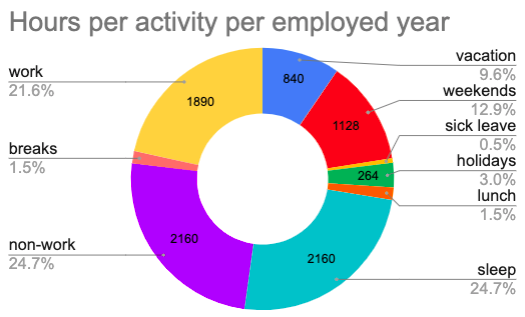
\includegraphics[width=0.8\textwidth]{images/hours_per_activity_per_employed_year}
    \caption{Hours of ``work'' per year when accounting for the rest of life. Assumes 5 weeks of vacation, 2 days of sick leave, and 11 holidays.}
    % footnotes in caption is not recommended; see https://texfaq.org/FAQ-ftncapt
    % however it can be done; see https://stackoverflow.com/questions/67621322/footnote-in-caption-of-figure-on-latex
    \label{fig:hours_per_year}
\end{figure}

Fig~\ref{fig:hours_per_year}
\footnote{\href{https://docs.google.com/spreadsheets/d/1ZaOZZXWkEzX4fFltUdlR4A6ENrAXnkzTW4YrjA4tDO8/edit?usp=sharing}{source for calculations}}

\ \\

\textbf{Less creativity}\\
See \S\ref{sec:innovation} for notes on innovation

\ \\

% https://graphthinking.blogspot.com/2017/04/growth-of-bureaucracy.html
\textbf{The larger a hierarchy, the ratio of workers to managers gets worse} \\

As complexity and workload increase, the number of staff needed increase. To facilitate coordination, managers arise. The amount of work being done in a bureaucracy can be small compared to the number of participants.

In Fig.~\ref{fig:growth_of_bureaucracy}a, the ratio of workers to participants is 3:3=1. When a manager is added, the ratio is 3:4 = 0.75. Adding a second team with dedicated management puts the ratio at 6:9=0.66. Finally, with a dedicated administrative team (ie HR, accounting), the ratio is 6:13=0.46.

    \begin{figure}
        \centering
        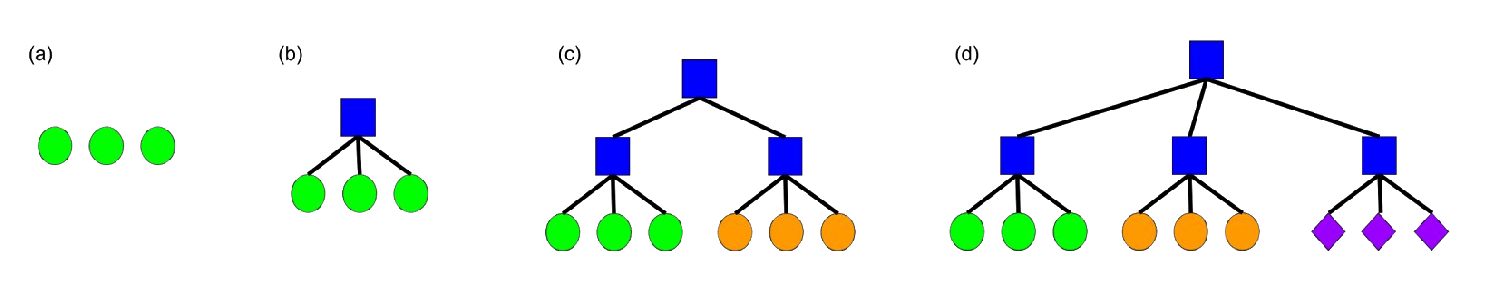
\includegraphics[width=1\textwidth]{images/growth-of-bureaucracy.pdf}
        \caption{growth of an organization as complexity and workload increase. a: three technical workers (green dots); b: administrative functions are delegated to a administrative assistant or manager (blue square); c: as complexity and scale grows, a new technical team (orange dots) is brought in which has their own manager; d: administrative work is delegated to a dedicated team of non-technical staff (purple diamonds).}
        \label{fig:growth_of_bureaucracy}
    \end{figure}

\ \\

\textbf{Each person in a bureaucracy has multiple roles} To limit the expansion of the bureaucracy. The multiple roles come from multiple relationships necessary to span an organization larger than \href{https://en.wikipedia.org/wiki/Dunbar\%27s_number}{Dunbar's number}. 

\ \\

\textbf{Bureaucracy is inefficient and wasteful}\\
Can you explain a pareto frontier for multiple objectives like speed, cost, accuracy?

Because decisions by bureaucrats are subjective, there is significant risk of being wrong or being called out by others as being wrong. Therefore, a motive to cover your ass for decisions made. Unnecessary work is carried out. 

Different participants have different motives, and the aggregation needed for coordination is inefficient regardless of what metric efficiency is measured against.

Another example: Inefficiency of changing the requirements on a project partway through. If an objective quantitative measure were available, the ROI could be determined. 

Efficiency is typically assessed from the perspective of a serial process -- a single worker could accomplish this task faster, so why involve 10 people and get a slower, more burdensome result? The Mythical Man Month manifests \href{https://en.wikipedia.org/wiki/Amdahl\%27s_law}{Amdahl's law}. Dividing a task among 10 people does not make the task 10x quicker. It's not valid to expect that a task which takes 1 person 1 hour to perfectly scale so 10 people should be able to accomplish 10 results in 1 hour.

Inefficiency of process is similar. I need to file a request to replace the lightbulb in my office. Compared to the serial ``I'll just replace the lightbulb myself by running to the hardware store and purchasing one."

The excess resources characterized as waste are similarly driven by the serial-based assessment of what one person would require to carry out the task. 

\ \\

% https://graphthinking.blogspot.com/2020/07/scope-creep-is-experienced-differently.html
\textbf{Scope creep} \\
The customer wants more, and the exploration of what's possible is exciting (a positive experience).

The creator hears more work. This implies a few trade-off options, all of which are negative for one or both parties.
\begin{itemize}
    \item sticking with the original terms (telling the customer "no", which is negative for both parties)
    \item re-negotiation for additional compensation (a burden to both parties)
    \item the programmer doing more for the same pay, which means less money per effort (yielding a less happy programmer)
    \item decreasing existing efforts to fit the additional new requirements (yielding a less happy customer)
    \item even if the programmer is getting paid by the hour, additional work means the end product will be delayed to accommodate additional features (yielding a less happy customer)
\end{itemize}

\ \\

% https://graphthinking.blogspot.com/2020/09/why-migrating-from-current-to-new.html
\textbf{Migrating technologies} \\
The person implementing the transition has to be educated in both the old and new technology. 
the legacy code has to be migrated to the new implementation
convincing stakeholders; may require synchronization
difficulty scales with the number of stakeholders 